

\documentclass[notitlepage,pra,10pt,aps]{revtex4-2}

\usepackage{geometry}
%\usepackage[hmargin=0.69in, vmargin=0.75in] {geometry}
\geometry{letterpaper}
%\usepackage{fullpage}
%\topmargin 0cm
\usepackage{bm}
\usepackage{float}
\usepackage{graphicx}
%\usepackage{epsfig}
\usepackage{amsfonts}
\usepackage{amsmath}
\usepackage{amssymb}
\usepackage{color}
%\usepackage{ulem}
\usepackage[colorlinks=true, citecolor= magenta]{hyperref}
\usepackage{epstopdf}
\usepackage{rotating}
\usepackage{natbib}
\usepackage[section]{placeins}
\usepackage{mdwlist}
\usepackage{lipsum}
\usepackage[caption=false, position=t,singlelinecheck=off]{subfig}

\newcommand{\com}[1]{{\color{blue}#1}}
\newcommand{\rev}[1]{{\color{red}#1}}
\newcommand {\be}{\begin{equation}}
\newcommand {\ee}{\end{equation}}
\newcommand{\ket}[1]{|#1\rangle}
\newcommand{\bra}[1]{\langle#1|}
\newcommand{\expect}[1]{\langle#1\rangle}
\newcommand{\braket}[2]{\langle#1|#2\rangle}
\newcommand{\ketbra}[2]{|#1\rlap{/}\backslash#2|}
\abovedisplayskip=6pt
\abovedisplayshortskip=0pt
\belowdisplayskip=6pt
\belowdisplayshortskip=6pt





\begin{document}

\title{Numerical integration of stochastic differential equations}
\author{Gerasimos Angelatos, Zachary Hervieux-Moore}
\affiliation{}
\maketitle
\tableofcontents
\pagenumbering{gobble}
%\addtocounter{page}{-1}
\pagenumbering{arabic}

\section{Introduction and background}

\subsection{Motivation}
% course covered odes and stuff in detail
% not much SDE stuff
% non differentialbility causes problems
%why interested in SDEs:
% used to model lots of systems
% solve fokker plank by simulating SDE
% many techni
In this course, we studied algorithms such as Runge-Kutta and Adams-Bashforth for solving systems of ordinary differential equations (ODEs).  However, in our research we occasionally encounter stochastic differential equations (SDEs): these models describe a wide variety of phenomena, from financial systems to quantum measurement.  Generally, any system whose evolution is continuous and has a non-deterministic evolution can be described by a set of SDEs.  This is equivalent to saying the probability density function of such a system obeys a Fokker-Plank equation (FPE), and indeed, the ability to map a FPE to an equivalent set of SDEs is a powerful solution method, regularly exploited in quantum optics \cite{Carmichael1999}, to treat FPEs which are otherwise difficult to solve.

However, the solution of SDEs, both numerically and even analytically, is considerably different than their deterministic counterparts.  All but the most simple algorithms for ODEs cannot be directly adapted to their stochastic counterparts because of the non-differentiability of the noise portion of their evolution.  Furthermore, these algorithms when adapted to SDEs result in a lower order of convergence.
There are only a few straightforward and broadly applicable algorithms for the solution of general systems of SDEs, which we present in this report. In addition, there are no widely-used python packages or libraries of SDE algorithms, and a naive attempt at solving a set of SDEs, for the reasons presented above, often ends in failure.  In this report, we consider the convergence and stability of three popular algorithms for solving SDEs:  Explicit Euler, Milstein, and Semi-Implicit Euler.  After presenting a background on SDEs, and describing each algorith, we discuss, evaluate and compare their convergence and stability properties.  We also wrote our own python SDE integrator class as a part of this project, the documentation for which is found in the appendix

\subsection{The Weiner Process}
\label{subsec:Weiner}
%gaussian noise
%properties of weiner process
% stochastic integral

The most intuitive introduction of an SDE is through a Langavin equation, which describes the evolution of some variable subject to a fluctuating force, which in 1-dimension can be written:
\be
\frac{d x}{dt}=A(x, t) +B(x, t)\zeta(t) \label{eq:lang}
\ee
where $\zeta$ is a rapidly fluctuating random term, such that $\zeta(t)$ and $\zeta(t')$ are statistically independent \cite{Gardiner2004}.   $\zeta(t)$ is white noise, meaning it obeys a Gaussian probability distribution with zero mean $\expect{\zeta(t)}=0$ and correlation $\expect{\zeta(t)\zeta(t')}=\delta(t-t')$, meaning the force at one time is completely uncorrelated with any other time.  To quantify this white noise, we integrate Eq.~\eqref{eq:lang}, and since we expect it to be integrable
\be
W(t)=\int_0^t ds \zeta(s)
\ee
exists and is a continuous quantity.  Furthermore, by splitting the above integral at $t'<t$ we see that $\zeta(s)$ in each integral are statistically independent: $W(t')$ and $W(t)-W(t')$ are independent as well then and is a Markov process.  Indeed by calculating moments it can readily be seen that $W(t)$ is the Weiner process (often referred to as Brownian motion), with the steady state distribution  (for initial condition $p(W, t_0| 0, t_0)= \delta(W)$):
\be
p(W, t| 0, t_0)=[(2\pi)(t-t_0)]^{-\frac{1}{2}}e^{\frac{-W^2}{2(t-t_0)}} \label{eq:pwien}
\ee
with zero mean $\expect{{W}(t)}=0$ and  linearly growing variance \cite{Gardiner2004} $\expect{W(t)^2}=t-t_0$. The Weiner process can be thought of as the limit of a continuous-time random walk.


 If one breaks the Weiner process into increments (which we will do shortly when solving SDEs) ${\Delta W_i}=W(t_i)-{W}(t_{i-1})$, from Eq.~\eqref{eq:pwien} we have the joint probability density $p({\Delta W_n}; {\Delta W_{n-1}};\dots{\Delta W_0})=\prod_{i=1}^n(2\pi\Delta t_i)^{-\frac{1}{2}}e^{\frac{-{\Delta W}_i^2}{2\Delta t_i}}p(W_0, t_0)$ \cite{Gardiner2004}.  Since the joint probability can been factorized into a product of individual probabilities for each Wiener increment  ${\Delta W_i}$, the $\{ {\Delta W_i}\}$ are statistically independent from each other.  Using this independence of increments, it can be seen that
\be
 \expect{{W}(t){W}(s)}=\min(t, s). \label{eq:Wcov}
\ee
Lastly, the Wiener process is non-differentiable, since $\lim_{h\to 0} {\rm Prob}(|W(t+h)-W(t)|/h>k)=\lim_{h\to 0} 2\int_{kh}^\infty (2\pi h)^{-\frac{1}{2}}e^{\frac{-W^2}{2h}}dW = 1$.  Thus the derivative is infinite, since $\lim_{h\to 0} |W(t+h)-W(t)|/h$ is larger than any value of $k$.

Because of this non-differentiablity, we should instead consider the integral form of  Eq.~\eqref{eq:lang}:
\be
x(t)=x(0)+\int_0^t A(x(s), s)+\int_0^t B(x(s), s) dW(s). \label{eq:ilang}
\ee
where
\be
dW(t)=W(t+dt)-W(t)=\zeta(t)dt \label{eq:Winc}
\ee
is the Wiener increment.

%%%
\subsection{Ito calculus}
%%%
Now once the Wiener increment has been defined, the question immediately arises of how to evaluate a stochastic integral, such as the final term of Eq.~\eqref{eq:ilang}.  Defining the stochastic integral $S=\int f(t')dW(t')$ as the $n\to\infty$ limit of partial sums:
\be
S_n\sum_i^n f(\tau_i)\left(W(t_i)-W(t_{i-1})\right),
\ee
it is apparent that the value of this quantity depends on where $\tau_i$ falls in the interval $t_{i-1}\to t_i$.  The Ito calculus is defined by the choice $\tau_i=t_{i-1}$ so that the Ito stochastic integral is
\be
\int_{t_0}^t f(t')dW(t')=\lim_{n\to\infty} \sum_i^n f(t_{i-1})\left(W(t_i)-W(t_{i-1})\right) \label{eq:ItoInt}
\ee
where the limit above is technically the mean square limit, indicating that the mean of the sequence converges to this value.  For a non-anticipating (ie.e.~physical) function, $f(t)$ in the Ito integral will be statistically independent of the Weiner increment and since  $\expect{dW(t)}=0$
\be
\expect{\int_{t_0}^t f(t')dW(t')}=0 \label{eq:meandw}
\ee
Furthermore, a straightforward application of Eq.~\eqref{eq:Wcov} to Eq.~\eqref{eq:Winc} gives $\expect{dW(t)^2}=dt$. It is also straightforward to derive $\int f(t') dW(t')^2=\lim_{n\to\infty} \sum_i^n f(t_{i-1})\left(W(t_i)-W(t_{i-1})\right)^2=\lim_{n\to\infty} \sum_i^n f(t_{i-1})\Delta t_i=\int f(t') dt'$.     Since $dW(t')$ only appears under an integral, we can therefore make the identification for Ito calculus that
$
dW(t)^2=dt
$.  This can be quickly extended to multi-dimensional systems $d\mathbf{W}$ and using the statistical independence of components $dW_i(t)$ and $dW_j(t)$ we have
  \be
  dW_i(t)dW_j(t)=\delta_{ij}dt \quad \quad
  dW_i(t)^{2+n}=0  \label{eq:dw2}
  \ee

These results can be readily understood by treating $dW(t)$ as an infinitesimal of order $\frac{1}{2}$, thus  $dW(t)^2=dt$ and $dW(t)^{2+n}=0$ since it is an infinitesimal of order greater than 1.  Now that an understanding of the Wiener process has been developed, we can define the Ito SDE for a multidimensional stochastic quantity $\mathbf{x}(t)$
\be
d\mathbf{x}(t)=\mathbf{A}(\mathbf{x}, t)dt+\mathbf{B}(\mathbf{x}, t)d\mathbf{W}
\ee
solved by
\be
\mathbf{x}(t)=\mathbf{x}(t_0)+\int_{t_0}^t \mathbf{A}(\mathbf{x}, t')dt'+\int_{t_0}^t \mathbf{B}(\mathbf{x}, t)d\mathbf{W}(t').\label{eq:intsde}
\ee

From here we can calculate various moments of $\mathbf{x}(t)$ using Ito calculus or numerically integrate the above to solve for sample trajectories using the algorithms discussed in the next section.  Since $dW$ is an infinitesimal of order $\frac{1}{2}$, one cannot blindly apply standard calculus to stochastic quantities $\mathbf{x}(t)$.  Consider an arbitrary function $f(\mathbf{x}(t))$:
\begin{align}
df(\mathbf{x})=&f(\mathbf{x}+d\mathbf{x})-f(\mathbf{x})=\partial_{x_i}f(\mathbf{x})dx_i +\frac{1}{2}\partial_{x_i}\partial_{x_j}f(\mathbf{x})dx_idx_j+\dots \nonumber \\
=&\partial_{x_i}f(\mathbf{x})\left(A_i+B_{ij}dW_j\right)+\frac{1}{2}\partial_{x_i}\partial_{x_j}f(\mathbf{x})\left[\mathbf{B}\mathbf{B}^T\right]_{ij}dt   \dots \label{eq:itocalc}
\end{align}
where in the both lines we drop all terms of order greater than $dt$ (note that we needed to continue the expansion to second order to produce all terms of order $dt$, unlike in standard calculus), and used Eq.~\eqref{eq:dw2} to yield the second line. Grouping terms we arrive at Ito's formula:
\be
df(\mathbf{x})=\left(A_i(\mathbf{x})\partial_{x_i}f(\mathbf{x})+ \frac{1}{2} \left[\mathbf{B}(\mathbf{x})\mathbf{B}^T(\mathbf{x})\right]_{ij}\partial_{x_i}\partial_{x_j}f(\mathbf{x})\right)dt
+B_{ij}(\mathbf{x})\partial_{x_i}f(\mathbf{x})dW_j \label{eq:itos}
\ee
 which is used to derive SDEs for arbitrary functions of a fundamental stochastic variable $\mathbf{x}(t)$

%%%
\subsection{Stratonovich calculus}
%%%

Equation \eqref{eq:ItoInt} is not the only choice of $\tau_i$ that can be used to evaluate the stochastic integral; the Stratonovich formulation evaluates the integrand at the center of the interval $\tau_i=\frac{t_i+t_{i-1}}{2}$:
\be
\int_{S,t_0}^t f(x(t'))dW(t')=\lim_{n\to\infty} \sum_i^n f(x(\frac{t_i+t_{i-1}}{2}))\left(W(t_i)-W(t_{i-1})\right) \label{eq:Stratint}
\ee
where the additional subscript $S$ differentiates this from an Ito stochastic integral. Now since $f(x(t'))$  is evaluated in the middle of the interval, it is no longer statistically independent of  $dW(t')$ and $\expect{\int_{t_0}^t f(x(t'))dW(t')}\neq0$. The connection between Stratanovich and Ito calculus can be seen by application of a discretized Eq.~\eqref{eq:itos} to Eq.~\eqref{eq:Stratint}:
\begin{align}
\lim_{n\to\infty} \sum_i^n f(x(\frac{t_i+t_{i-1}}{2}))\left(W(t_i)-W(t_{i-1})\right)=& \lim_{n\to\infty} \sum_i^n f(x(t_{i-1}))\left(W(t_i)-W(t_{i-1})\right) \nonumber \\
+&\frac{1}{2}\sum_i^n B(x(t_{i-1}))\partial_x B(x(t_{i-1}))(t_i-t_{i-1})\nonumber
\end{align}
The first term on the right side is the Ito integral, and the second is a standard integral over time and can thus be  grouped in with the integration over the drift vector.  In general, an Ito SDE $d\mathbf{x}=\mathbf{A}^{\rm Ito}dt+\mathbf{B}d\mathbf{W}$ is equivalent to the Stratonovich SDE $d\mathbf{x}=\mathbf{A}^{\rm strat}dt+\mathbf{B}d\mathbf{W}$ with $\mathbf{A}^{\rm strat}=\mathbf{A}^{\rm Ito}+\mathbf{A}^{\rm corr}$, with
\be
{A}^{\rm corr}_i=-\frac{1}{2}\sum_{jk}B_{kj}\partial_{x_k}B_{ij}
\label{eq:Acorr}
\ee
 The Stratonovich formulation may seem like a lot of unnecessary work, but it has one significant advantage: numerical convergence and stability, as will be noted later.  In addition, from Eqs.~\eqref{eq:Acorr} and \eqref{eq:itos}, one can show that the Stratonovich formulation of stochastic calculus obeys the same rules for a change of variables as ordinary calculus:
\be
df(\mathbf{x})=\left(\mathbf{A}^{\rm strat}dt+\mathbf{B}d\mathbf{W}\right)f'(\mathbf{x})
\ee


\section{Algorithms to integrate stochastic differential equations}

\subsection{Explicit Euler algorithm}

\subsection{Milstein algorithm}

\subsection{Semi-Implicit Euler}

\section{Convergence and Stability}
\subsection{Strong and weak convergence}

Just as probability theory has multiple notions of convergence (in distribution, in probability, etc.), there are two notions of convergence in the numerical analysis of stochastic differential equations. The first is strong convergence which is completely analogous to the convergence in $L^1$ norm of probability. Something is strongly convergent if:

\begin{gather*}
  \lim_{\delta t \rightarrow 0} \mathbb{E} \left[ \lvert X_T - X_T^{\delta t} \rvert \right] = 0
\end{gather*}

In words, it is strongly convergent if the expected absolute difference between the actual process, $X$, and the process generated by a numerical algorithm with time step $\delta t$, $X^{\delta t}$,  agree with each other at the end time point $T$. Note that this is a very strong statement about the generation of the path trajectories. It essentially says that the algorithm generates paths identical to the actual process if the time step becomes small enough. Thus, strong convergence is a necessity if you need a numerical scheme that keeps the paths along similar trajectories as the underlying process. To measure the rate of convergence, we say that it is strongly convergent with order $\gamma$ if

\begin{gather*}
  \mathbb{E} \left[ \lvert X_T - X_T^{\delta t} \rvert \right] \leq O(\delta t)^\gamma
\end{gather*}

The second notion of convergence is weak convergence which is similar to the convergence in distribution of probability. Something is weakly convergent if:

\begin{gather*}
  \lim_{\delta t \rightarrow 0} \left\lvert \mathbb{E} \left[ g(X_T) \right] - \mathbb{E} \left[ g(X_T^{\delta t}) \right] \right\lvert = 0 \text{ for all polynomial } g
\end{gather*}

Loosely speaking, it is weakly convergent if the expected absolute difference between the moments of the actual process and the moments of process generated by a numerical algorithm with time step $\delta t$, agree with each other at the end time point $T$. This is much weaker than the previous type of convergence. We allow for the numerical algorithm to deviate from the actual process as long as the mean remains unchanged. Intuitively, if we had a Gaussian process, we might expect an algorithm to introduce more variance. If it did so, it would no longer converge strongly but still converges weakly. To measure the rate of convergence, we say that it is weakly convergent with order $\gamma$ if

\begin{gather*}
  \left\lvert \mathbb{E} \left[ X_T \right] - \mathbb{E} \left[ X_T^{\delta t} \right] \right\lvert \leq O(\delta t)^\gamma
\end{gather*}

In practice, requiring strong convergence is too much. Chiefly, it is often the case that the actual distribution of the process is unknown. However, we may know the moments of the process in which case weak convergence is readily available to test against. Also, in applications that care only about the end point such as European options pricing, we do not need strong convergence. This is often the case where we do not care how a particle gets to a position as long as the final position is accurate.

For completeness, the rates of convergences for the algorithms discussed are shown bellow:

\begin{center}
  \begin{tabular}{c | c | c}
    \textbf{Algorithm} & \textbf{Strong Rate} & \textbf{Weak Rate} \\
    \hline
    \text{Euler} & 1/2 & 1 \\
    \hline
    \text{Semi Implicit} & 1/2 & 1 \\
    \hline
    \text{Milstein} & 1 & 1
  \end{tabular}
\end{center}

\subsection{Stability}

\section{Results}
  \subsection{Geometric Brownian Motion}
  The first case study of the different algorithm we considered was Geometric Brownian Motion (GBM). GBM is the system that satisfies the following SDE:

  \begin{gather*}
    d S_t = \mu S_t dt + \sigma S_t d W_t
  \end{gather*}

  This process has multiplication noise and so it tends to be unstable. Furthermore, we know the solution of this SDE is

  \begin{gather*}
    S_t = S_0 e^{(\mu - \frac{\sigma^2}{2})t + \sigma W_t}
  \end{gather*}

  Recall that the noise term is normal and hence $S_t$ is a lognormal distribution with parameters:
  \begin{gather*}
    \mu_{dist} = (\mu - \frac{\sigma^2}{2})t + \log(S_0) \\
    \sigma_{dist} = \sigma \sqrt{T}
  \end{gather*}

  Where $\mu_{dist}$ and $\sigma_{dist}$ are the parameters of the lognormal distribution and $\mu$ amd $\sigma$ are parameters of the SDE. Below is a plot of sample paths for $\mu = -5$, $\sigma = 1$, and $S_0 = 10$.

  \begin{figure}[H]
    \centering
      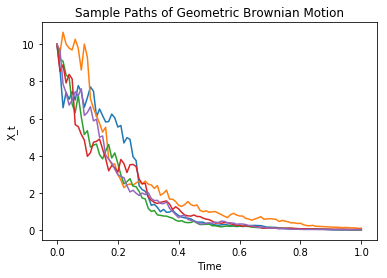
\includegraphics[width=0.7\textwidth]{sample_paths_gbm.png}
    \caption{Five sample paths of GBM with parameters $\mu = -5$, $\sigma = 1$, and $S_0 = 10$}
  \end{figure}

  See how this function starts pretty volatile but decreases in variance as it approaches 0 as the multiplicative noise term becomes smaller and smaller. It also tends towards zero because our $\mu$ is negative. Otherwise, it would tend to infinity and be unstable. To confirm that our sample paths follow GBM, we generated 1000 paths and compared the empirical distribution to the expected analytical distirubtion. This is show in the figure below.

  \begin{figure}[H]
    \centering
      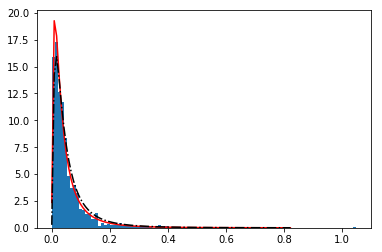
\includegraphics[width=0.7\textwidth]{lognormal_gbm.png}
    \caption{The histogram of 1000 sample path endpoints. The red line is the estimated log normal. The dotted black line is the theoretical distribution.}
  \end{figure}

  We now compare the convergence rate of GBM across the various algorithms. To highlight differences, we used a GBM model with parameters $\mu = -10$, $\sigma = 1$, and $S_0 = 100$. In the three following graphs, the x-axis is a log scale.

  \begin{figure}[H]
    \centering
      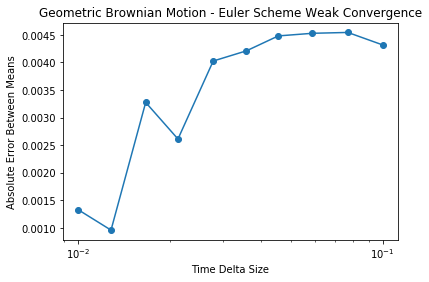
\includegraphics[width=0.7\textwidth]{gbm_euler.png}
    \caption{GBM Weak Convergence for the Euler Method. Absolute Error of Means vs. Time Step Size. Dotted line has slope 1.}
  \end{figure}

  \begin{figure}[H]
    \centering
      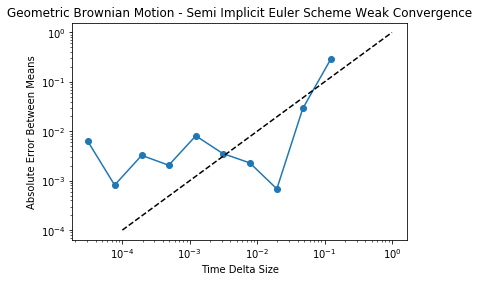
\includegraphics[width=0.7\textwidth]{gbm_semi.png}
    \caption{GBM Weak Convergence for the Semi Implicit Euler Method. Absolute Error of Means vs. Time Step Size. Dotted line has slope 1.}
  \end{figure}

  \begin{figure}[H]
    \centering
      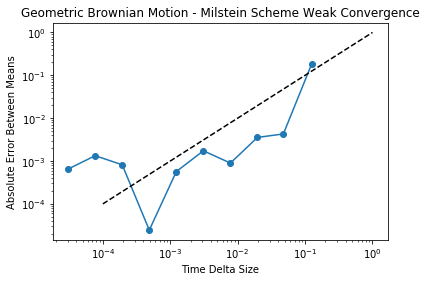
\includegraphics[width=0.7\textwidth]{gbm_milstein.png}
    \caption{GBM Weak Convergence for the Milstein Method. Absolute Error of Means vs. Time Step Size. Dotted line has slope 1.}
  \end{figure}

  We note here that the actual convergence of the algorithms matches pretty similarly to the . All three seem to track the line with slope 1 on the log-log plot which implies that the convergence rate is 1. The only method in question is the semi implicit Euler scheme. We hypothesize the flattening of the curve is due to it reaching some lower bound earlier than the others.

  \subsection{Ornstein-Uhlenbeck Process}

  For the second case study, we considered the Ornstein-Uhlenbeck (OU) Process. The OU process has the following dynamics

  \begin{gather*}
    d X_t = \mu(\theta-X_t) dt + \sigma dW_t
  \end{gather*}

  This process differs from GBM in that the noise is only additive. Intuitively, this process tends towards $\theta$ as time goes on. The rate at which it tends there is dictated by $\mu$. The solution of the OU process is given by

  \begin{gather*}
    X_t = X_0 e^{-\mu t}+ \theta(1-e^{-\mu T}) + \sqrt{\frac{\sigma}{\mu} (1-e^{-2 \mu t})} W_t
  \end{gather*}

  Where this is clearly normal with parameters

  \begin{gather*}
    \mu_{dist} = X_0 e^{-\mu t}+ \theta(1-e^{-\mu T})  \\
    \sigma_{dist} = \sqrt{\frac{\sigma}{\mu} (1-e^{-2 \mu t})}
  \end{gather*}

  Where $\mu_{dist}$ and $\sigma_{dist}$ are the parameters of the lognormal distribution and $\mu$ amd $\sigma$ are parameters of the SDE. Below is a plot of sample paths for $\mu = 0.01$, $\theta =1$, $\sigma = 0.01$, and $X_0 = 0$.

  \begin{figure}[H]
    \centering
      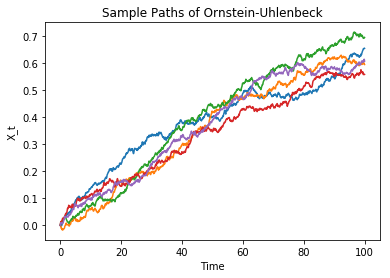
\includegraphics[width=0.7\textwidth]{sample_paths_ou.png}
    \caption{Five sample paths of GBM with parameters $\mu = 0.01$, $\theta =1$, $\sigma = 0.01$, and $X_0 = 0$}
  \end{figure}

  Generating 1000 sample paths and fitting them to a normal yields the following comparison to the expected normal distribution

  \begin{figure}[H]
    \centering
      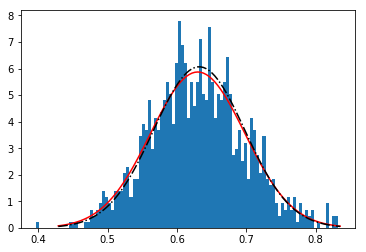
\includegraphics[width=0.7\textwidth]{normal_ou.png}
    \caption{The histogram of 1000 sample path endpoints. The red line is the estimated normal. The dotted black line is the theoretical distribution.}
  \end{figure}

  Finally, we compare the different schemes and their convergence rates. For the OU process, we are able to analytically determin $\lvert X_T - X_T^{\delta t} \rvert$ because everything is a Gaussian and thus the absolute value of the difference is a well known folded normal distribution. For the Euler scheme, we get that the convergence rates for both strong and weak seems to equal exactly 1.

  \begin{figure}[H]
    \centering
      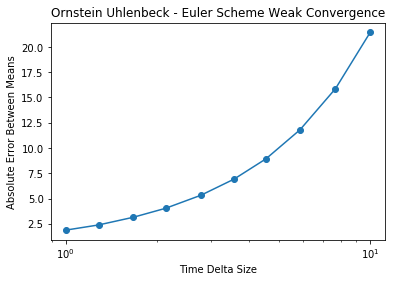
\includegraphics[width=0.7\textwidth]{ou_weak_euler.png}
    \caption{OU Weak Convergence for the Euler Method. Absolute Error of Means vs. Time Step Size. Dotted line has slope 1.}
  \end{figure}

  \begin{figure}[H]
    \centering
      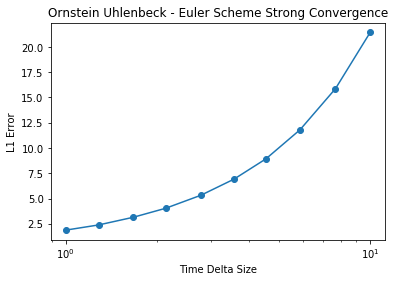
\includegraphics[width=0.7\textwidth]{ou_strong_euler.png}
    \caption{OU Strong Convergence for the Euler Method. Absolute Error of Means vs. Time Step Size. Dotted line has slope 1.}
  \end{figure}

  For the semi implicit Euler method, we get something of a different result. We get that the weak convergence rate is greater than 1, something close to 2. Whereas the strong convergence is 1. While this does not match the theory of 1 and 1/2, they do differ by a factor of 2. This might be explained by the fact that the OU process is in itself very convergent as it has many nice properties due to its Gaussian nature.

  \begin{figure}[H]
    \centering
      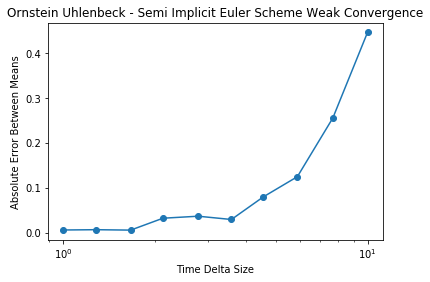
\includegraphics[width=0.7\textwidth]{ou_weak_semi.png}
    \caption{OU Weak Convergence for the Semi Implicit Euler Method. Absolute Error of Means vs. Time Step Size. Dotted line has slope 1.}
  \end{figure}

  \begin{figure}[H]
    \centering
      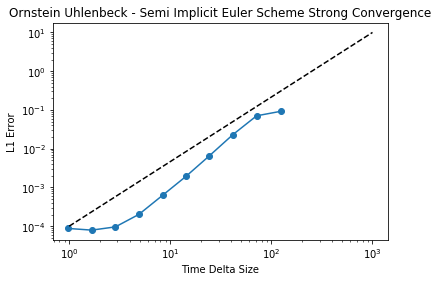
\includegraphics[width=0.7\textwidth]{ou_strong_semi.png}
    \caption{OU Strong Convergence for the Semi Implicit Euler Method. Absolute Error of Means vs. Time Step Size. Dotted line has slope 1.}
  \end{figure}

  Finally, for the Milstein algorithm, we get again that both convergence rates equal 1.

  \begin{figure}[H]
    \centering
      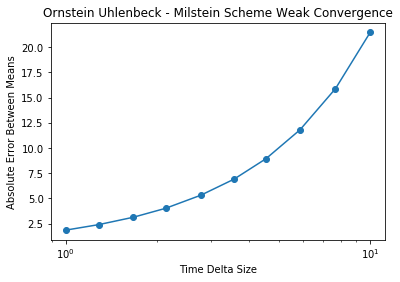
\includegraphics[width=0.7\textwidth]{ou_weak_milstein.png}
    \caption{OU Weak Convergence for the Milstein Method. Absolute Error of Means vs. Time Step Size. Dotted line has slope 1.}
  \end{figure}

  \begin{figure}[H]
    \centering
      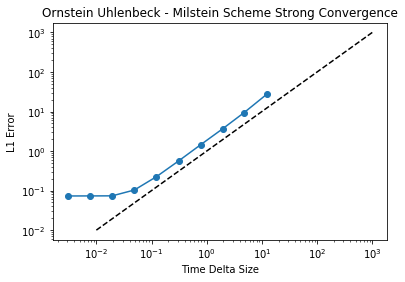
\includegraphics[width=0.7\textwidth]{ou_strong_milstein.png}
    \caption{OU Strong Convergence for the Milstein Method. Absolute Error of Means vs. Time Step Size. Dotted line has slope 1.}
  \end{figure}


\section{Conclusions}

To conclude, this project has been a cursory overview of the numerical methods literature on stochastic differential equations. If one wanted to explore the field in depth, there are more advanced algorithms taking into account second order effects. Another immediate extention of the work on this project is to apply the algorithms to multidimensional systems and see which ones provide the best results. With regards to implementation detail, the work on this project yielded a few tangential avenues to explore.

One of the possible avenues is curve fitting. Curve fitting was done to compare the convergence rates of the various algorithms. In general, the problem of fitting a distribution to a dataset is very hard. Even if one knows the form of the distribution, the problem of finding the best parameters could be nonconvex. This is illustrated by a simple mixture of Gaussians. However, even if one has a convex problem, the classic problems of numerical analysis apply. What are the best schemes to minimize the objective, are these gradient steps stable (i.e. do we invert a matrix), how does one handle distributions that yield extremely large numbers? All of these concerns have to be addressed before attempting to fit a curve. Fortunately, in our cases, we studied equations with well known and well behaved solutions. In general, this area is ripe for exploration.


\bibliographystyle{ieeetr}
\bibliography{reprefs}
\end{document}

